\documentclass[aspectratio=169]{beamer}
\usepackage[utf8]{inputenc} % codificacao de caracteres
\usepackage[T1]{fontenc}    % codificacao de fontes
\usepackage[brazil]{babel}  % idioma
\usepackage{graphics,amssymb,amsfonts,amsmath}
\usepackage{tikz}
\usepackage{enumerate,hyperref}
\usepackage{palatino}	% Fonte sem serifa
\usepackage{ragged2e}	% Paragrafo justificado
%\usepackage{minted}	% Highlight para codigos de programacao
\usepackage{booktabs} % tabelas
\usepackage{multicol}
\usepackage{multirow}
%\usepackage[table]{xcolor}


% Veja mais temas e cores em http://www.hartwork.org/beamer-theme-matrix/
\usetheme{Montpellier}         % tema
\usecolortheme{orchid}      % cores
\usefonttheme[onlymath]{serif} % fonte modo matematico
% Colocando numero de paginas no slide
\setbeamertemplate{footline}[frame number]



\DeclareGraphicsExtensions{.pdf,.JPG,.png} % compilamos apenas com pdflatex
\graphicspath{{./figuras/}} % caminho onde as figuras estarao disponiveis




% ---------------------------------------------------------------------------- %
% T�tulo                                                                       %
% ---------------------------------------------------------------------------- %

\title[\sc{Teoria de Circuitos Eletrônicos 1}]{\LARGE Aula 3: Methods of Analysis of Resistive Circuits (Mesh Current)}
\author[Prof. Marcelino Andrade]{Prof. Marcelino Andrade}
\institute{Faculdade UnB Gama} % opcional
\date{\today}

\begin{document}
\justifying % Paragrafo justificado
\pagebreak

\begin{frame}
  \titlepage
\end{frame}


% ----------------- NOVO SLIDE --------------------------------
\begin{frame}{Contents\newline}

\tableofcontents
\begin{center}	
     		Introduction to Electric Circuits 9th Edition by James A. Svoboda, Richard C. Dorf			
\end{center}	
\end{frame}

% ----------------- NOVA SECÇÂO -----------------------------
\section{Introduction (4.1)}
% ----------------- NOVO SLIDE --------------------------------
\begin{frame}[fragile]
	\frametitle{Introduction}
		\begin{tabular}{cc}
			\begin{columns}
				\begin{column}{1\textwidth}  %%<--- here
					In this chapter, we consider two methods for writing a smaller set of simultaneous equations:	\newline
		
					\begin{itemize}
						\item[$\clubsuit$] \scalebox{1.5}{The node voltage method.}
						\item[$\clubsuit$] \scalebox{1.5}{The mesh current method	.}						
					\end{itemize}
					.\newline To analyze an electric circuit, we write and solve a set of equations. We apply Kirchhoff’s current and
					voltage laws to get some of the equations. This method works well for small circuits, but the set of equations can get quite large for even
					moderate-sized circuits.
				\end{column}
			\end{columns}
		
	\end{tabular}
\end{frame}

% ----------------- NOVA SECÇÂO -----------------------------
\section{Mesh Current Analysis with Independent Voltage Sources (4.5)}
% ----------------- NOVO SLIDE --------------------------------
\begin{frame}[fragile]
	\frametitle{Mesh Current Analysis}
\begin{tabular}{c}
	\begin{columns}	\column{1\textwidth}
		A \textbf{mesh} is a loop that does not contain any other loops within it.
	\end{columns} \\
	\begin{columns}
		\begin{column}{0.5\textwidth}  %%<--- here
			\begin{center}
			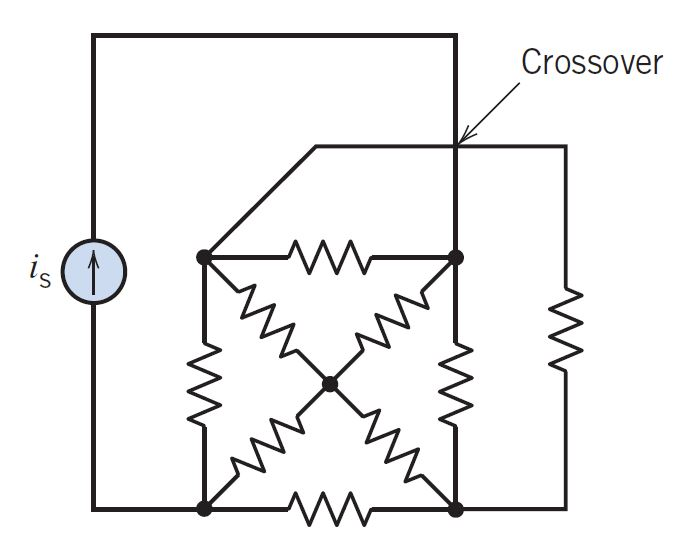
\includegraphics[width=.7\textwidth]{figura4_51.JPG}\\
			Nonplanar circuit with a crossover.	
			\end{center}
		\end{column}
		\begin{column}{0.5\textwidth}  %%<--- here
			\begin{center}
			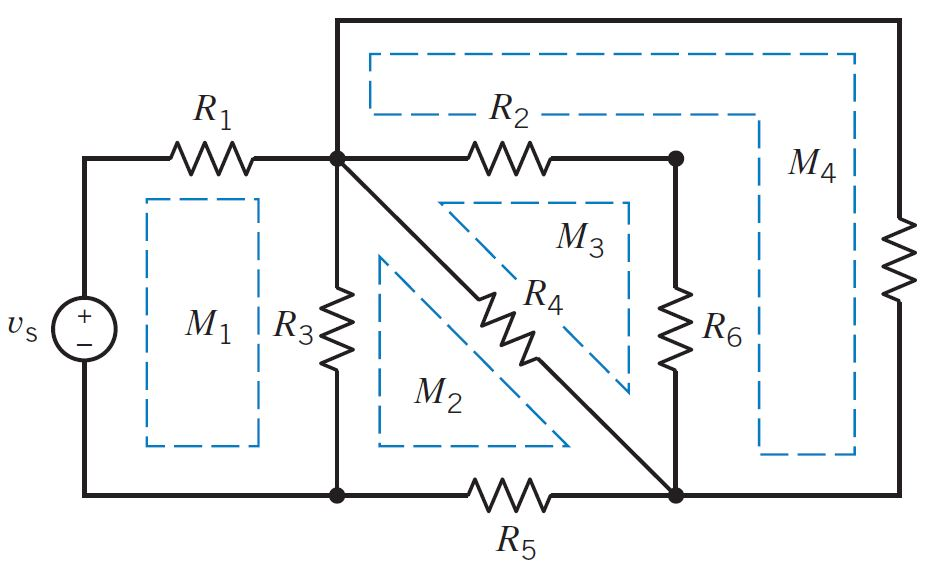
\includegraphics[width=.9\textwidth]{figura4_52.JPG}\\
			Circuit with four meshes.
			\end{center}	
		\end{column}
	\end{columns}
\end{tabular}
\end{frame}
% ----------------- NOVO SLIDE --------------------------------
\begin{frame}[fragile]
	\frametitle{Mesh Current Analysis}
\begin{tabular}{r}
	\begin{columns}	\column{1\textwidth}
		A \textbf{mesh} is a loop that does not contain any other loops within it.
	\end{columns} \\
	\begin{columns}
		\begin{column}{0.4\textwidth}  %%<--- here
			\begin{center}
			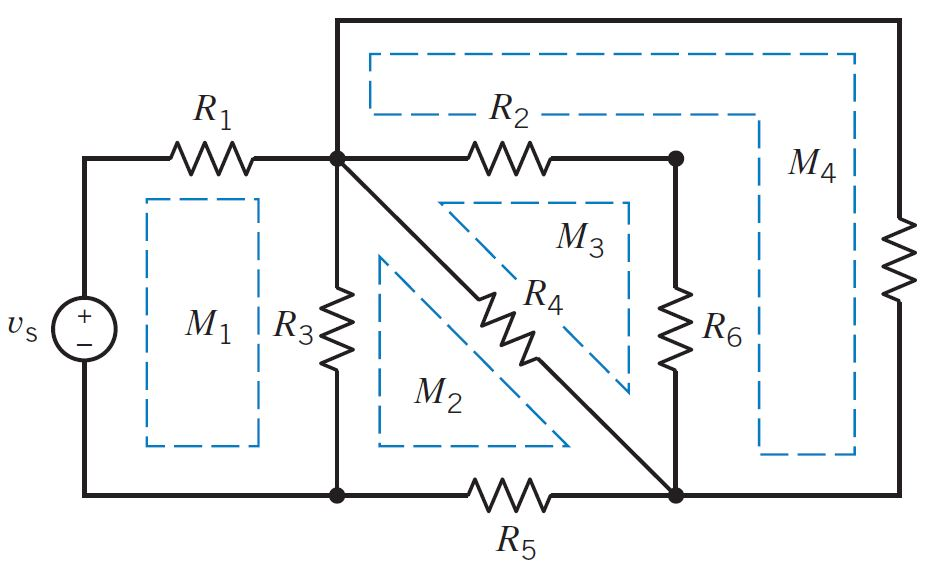
\includegraphics[width=1.1\textwidth]{figura4_52.JPG}\\
			Circuit with four meshes.	
			\end{center}
		\end{column}
		\begin{column}{0.6\textwidth}  %%<--- here
			{To write a set of mesh equations, we do two things:}\\
			\begin{itemize}
				\item[$\clubsuit$] {Express element voltages as functions of the mesh currents.}
				\item[$\clubsuit$]  {Apply Kirchhoff’s voltage law (KVL) to each of the meshes of the circuit.}
			\end{itemize}
		\end{column}
	\end{columns}
\end{tabular}
\end{frame}

% ----------------- NOVO SLIDE --------------------------------
\begin{frame}[fragile]
	\frametitle{Mesh Current Analysis}
\begin{tabular}{r}
	\begin{columns}	\column{1\textwidth}
	These equations expresses the currents $i_{b},\ -3\ $ and $i$ as a function of the mesh currents$\ i_{1}$ and $i_{2}$.
	\end{columns} \\
	\begin{columns}
		\begin{column}{0.33\textwidth}  %%<--- here
	%		\begin{center}
			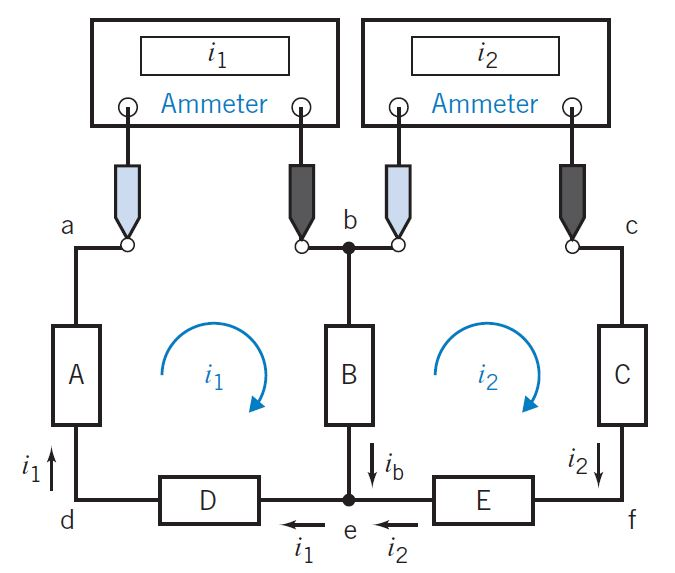
\includegraphics[height=4cm]{figura4_53b.JPG}\\
			\begin{equation}
				 i_{b}=i_{1}-i_{2}
			\end{equation}	
	%	\end{center}			

		\end{column}
		\begin{column}{0.33\textwidth}  %%<--- here
			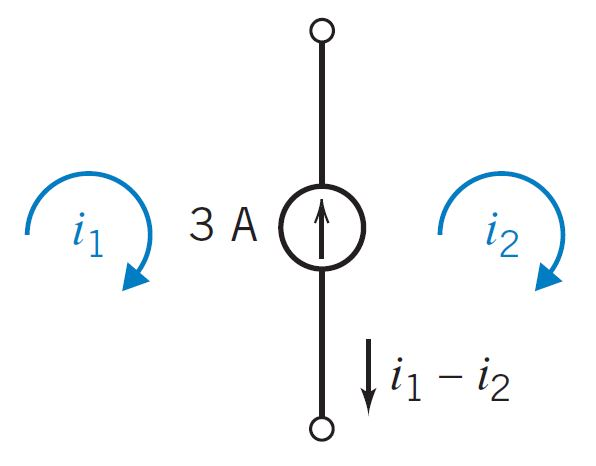
\includegraphics[height=4cm]{figura4_54b.JPG}\\
			\begin{equation}
				 -3=i_{1}-i_{2}
			\end{equation}			
		\end{column}
		\begin{column}{0.33\textwidth}  %%<--- here
			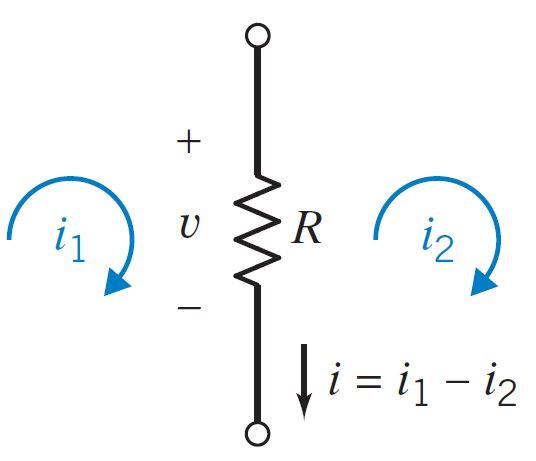
\includegraphics[height=4cm]{figura4_54c.JPG}\\
			\begin{equation}
				 v=R(i_{1}-i_{2})
			\end{equation}
		\end{column}
	\end{columns}
\end{tabular}
\end{frame}

% ----------------- NOVO SLIDE --------------------------------
\begin{frame}[fragile]
	\frametitle{Mesh Current Analysis with Independent Voltage Sources}
\begin{tabular}{r}
	\begin{columns}	\column{1\textwidth}
		Next, let’s write mesh equations to represent the circuit shown.
	\end{columns} \\
	\begin{columns}
		\begin{column}{0.3\textwidth}  %%<--- here
	
			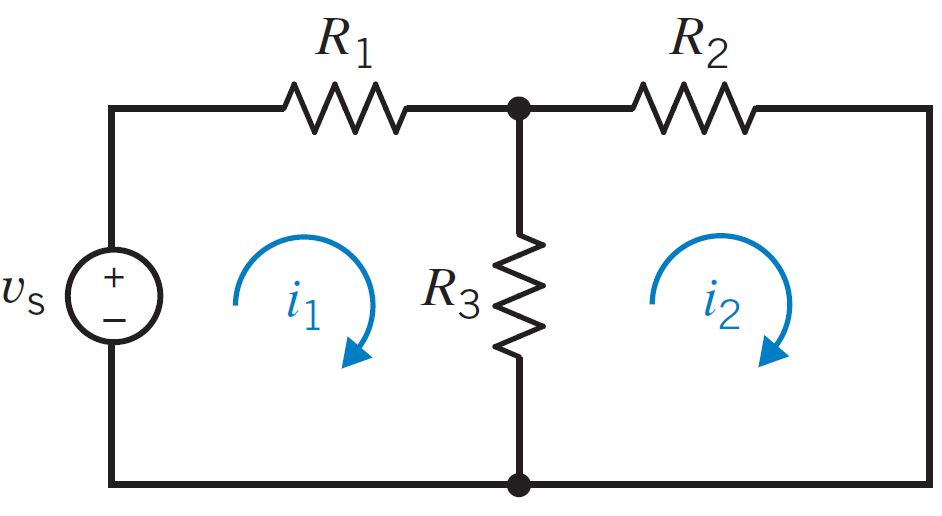
\includegraphics[height=2.8cm]{figura4_55a.JPG}\\
			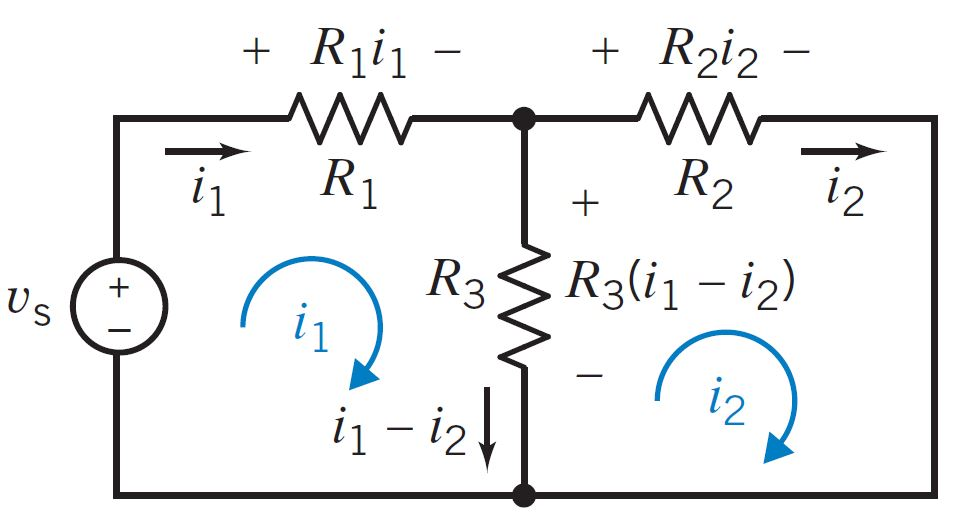
\includegraphics[height=2.8cm]{figura4_55c.JPG}\\

		\end{column}
		\begin{column}{0.5\textwidth}  %%<--- here
			\begin{equation}
				 -v_{s}+R_{1}i_{1}+R_{3}(i_{1}-i_{2})=0
			\end{equation}		
			\begin{equation}
				- R_{3}(i_{1}-i_{2})+R_{2}i_{2}=0
			\end{equation}	
						\[ 
			\left[\begin{array}{cc}
			R_{1}+R_{3} & -R_{3} \\
			-R_{3} & R_{2}+R_{3} \end{array} \right]
			\left[\begin{array}{c}
			i_{1} \\
			 i_{2}\end{array} \right]= 
			\left[\begin{array}{c}
			v_{s} \\
			0  \end{array} \right]
			\]	
			
%	\begin{center}
\scalebox{0.9}{  If $ R_{1}=R_{2}=R_{3}= 1\Omega$ and $v_{s}=3V$, we have}
%\end{center}
	
	\[ 
			\left[\begin{array}{cc}
			2 & -1 \\
			-1 & 2 \end{array} \right]
			\left[\begin{array}{c}
			i_{1} \\
			 i_{2}\end{array} \right]= 
			\left[\begin{array}{c}
			3 \\
			0  \end{array} \right]
			\]
		%\begin{center}
	\scalebox{0.9}{then we have $i_{1}=2$ and $i_{2}=1$.}
		%\end{center}

	\end{column}

	\end{columns}
\end{tabular}
\end{frame}
% ----------------- NOVO SLIDE --------------------------------
\begin{frame}[fragile]
	\frametitle{Mesh Current Analysis with Independent Voltage Sources}

\begin{tabular}{ll}
	\begin{columns}
		\begin{column}{1\textwidth}  %%<--- here
		\textbf{EXERCISE 4.5-1} - Determine the value of the voltage measured by the voltmeter.\\
		\begin{center}
    			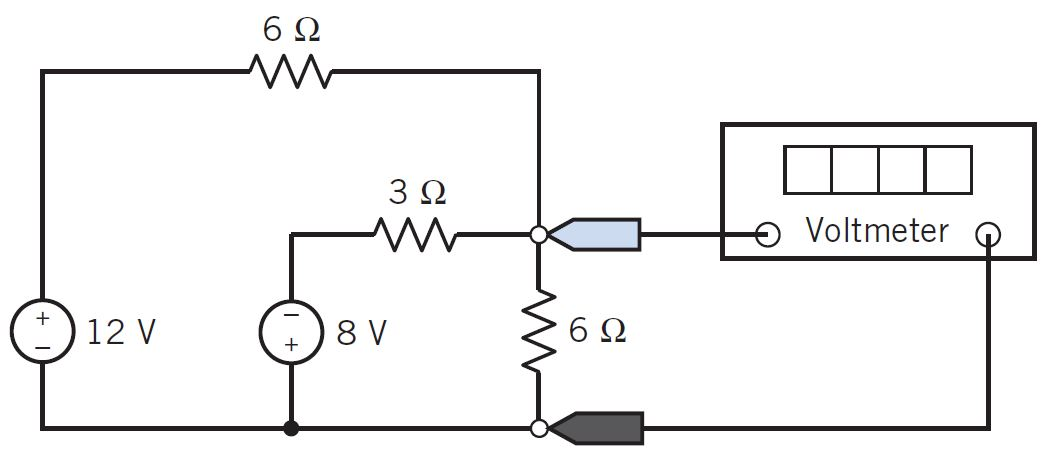
\includegraphics[width=.6\textwidth]{figuraE4_51.JPG}\\	
		\end{center}	
		\scalebox{0.8}{Answer: -1}
		\end{column}
	\end{columns}
\end{tabular}
\end{frame}

% ----------------- NOVA SECÇÂO -----------------------------
\section{Mesh Current Analysis with Current and Voltage Sources (4.6)}
% ----------------- NOVO SLIDE --------------------------------
\begin{frame}[fragile]
	\frametitle{Mesh Current Analysis with Current and Voltage Sources}


\begin{tabular}{ll}
	\begin{columns}[c]	\column{1\textwidth}
		Circuit with an independent voltage source and an independent current source.
	\begin{center}
{}
\end{center}
	\end{columns} \\
	\begin{columns}
		\begin{column}{0.5\textwidth}  %%<--- here
		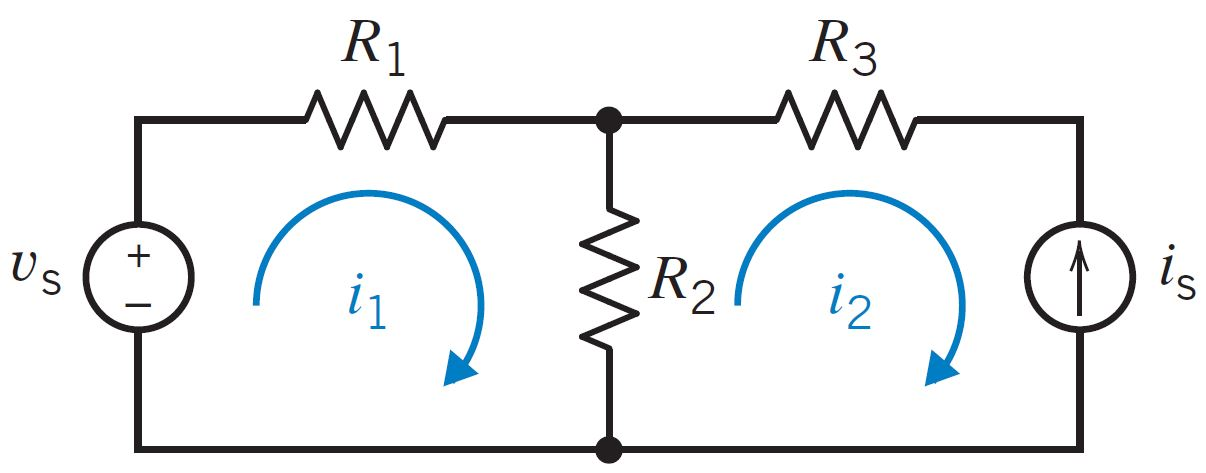
\includegraphics[width=1.2\textwidth]{figura4_61.JPG}\\	
	%	\scalebox{1}{Answer:$\ v_{a} = -4/3V\ and \  v_{b} = 4 V$}
		\end{column}
		\begin{column}{0.5\textwidth}  %%<--- here
			\begin{equation}
			 i_{2}=-i_{s}
			\end{equation}
			\begin{equation}
			-v_{s}+R_{1}i_{1}+R_{2}(i_{1}-i_{2})=0
			\end{equation}
			\begin{equation}
			i_{1}=\frac{v_{s}+R_{2}i_{2}}{R_{1}+R{2}}
			\end{equation}
			\begin{equation}
			i_{1}=\frac{v_{s}+R_{2}i_{s}}{R_{1}+R{2}}
			\end{equation}
		\end{column}
	\end{columns}\\

\end{tabular}

\end{frame}

% ----------------- NOVO SLIDE --------------------------------
\begin{frame}[fragile]

	\frametitle{Mesh Current Analysis with Current and Voltage Sources}
\begin{tabular}{ll}
	\begin{columns}[c]	\column{1\textwidth}
		Circuit with an independent current source common to both meshes.
	\end{columns} \\
	\begin{columns}
		\begin{column}{0.5\textwidth}  %%<--- here
		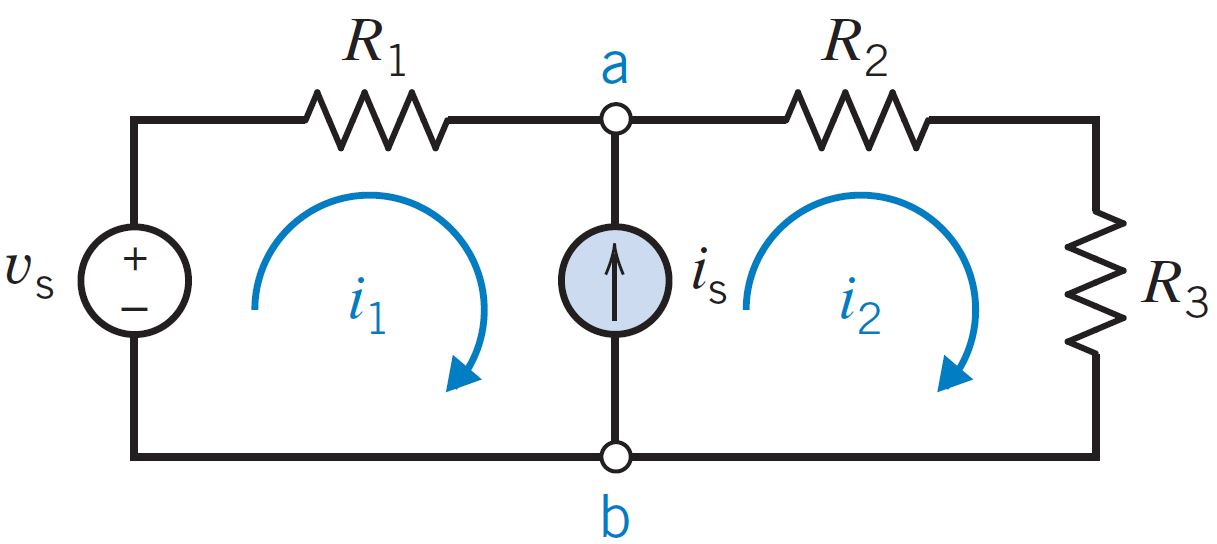
\includegraphics[width=1.2\textwidth]{figura4_62.JPG}\\	
	%	\scalebox{1}{Answer:$\ v_{a} = -4/3V\ and \  v_{b} = 4 V$}
		\end{column}
	\begin{column}{0.5\textwidth}  %%<--- here
			\begin{equation}
			i_{1}- i_{2}=-i_{s}
			\end{equation}
			\begin{equation}
			-v_{s}+R_{1}i_{1}+v_{ab}=0
			\end{equation}
			\begin{equation}
			-v_{ab}+R_{2}i_{2}+R_{3}i_{2}=0
			\end{equation}
			\begin{equation}
			-v_{s}+R_{1}i_{1}=-R_{2}i_{2}-R_{3}i_{2}
			\end{equation}
				\[ 
			\left[\begin{array}{cc}
			R_{1} & R_{2}-R_{3} \\
			1 & -1 \end{array} \right]
			\left[\begin{array}{c}
			i_{1} \\
			 i_{2}\end{array} \right]= 
			\left[\begin{array}{c}
			v_{s} \\
			-i_{s}  \end{array} \right]
			\]	
		\end{column}
	\end{columns}\\
\end{tabular}
\end{frame}
% ----------------- NOVO SLIDE --------------------------------


\begin{frame}[fragile]

	\frametitle{Mesh Current Analysis with Current and Voltage Sources}
\begin{tabular}{ll}
	\begin{columns}
		\begin{column}{1\textwidth}  %%<--- here
		\textbf{EXAMPLE 4.6-1} - Consider the circuit of Figure where $R_{1}=R_{2}= 1\Omega$ and
$R_{3}=2\Omega$. Find the three mesh currents\\
		\begin{center}
    			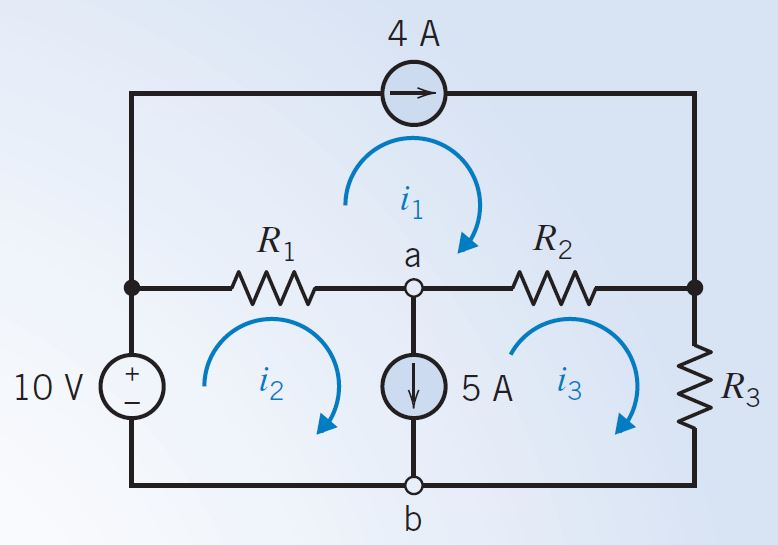
\includegraphics[width=.4\textwidth]{figura4_63.JPG}\\	
		\end{center}	
		\scalebox{0.8}{Answer: $i_{3}=\frac{13}{4}$ and $i_{2}=\frac{33}{4}$}
		\end{column}
	\end{columns}
\end{tabular}
\end{frame}
% ----------------- NOVO SLIDE --------------------------------
\begin{frame}[fragile]

\frametitle{Supermesh Current Analysis with Current and Voltage Sources}
\begin{tabular}{ll}
	\begin{columns}[c]	\column{1\textwidth}
		A \textbf{supermesh} is one larger mesh created from two meshes that have an independent or dependent current source in common.
	\end{columns} \\
	\begin{columns}
		\begin{column}{0.3\textwidth}  %%<--- here
		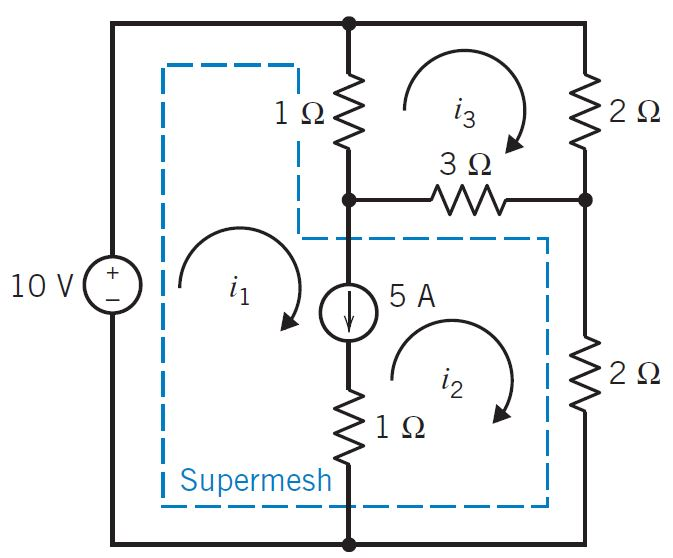
\includegraphics[width=1.2\textwidth]{figura4_64.JPG}\\	
	%	\scalebox{1}{Answer:$\ v_{a} = -4/3V\ and \  v_{b} = 4 V$}
		\end{column}
		\begin{column}{0.7\textwidth}  %%<--- here
			\begin{equation}
			current \ source: i_{1}- i_{2}=5
			\end{equation}
			\begin{equation}
			mesh \ 3: 2i_{3}-3(i_{2}-i_{3})-1(i_{1}-i_{3})=0
			\end{equation}
			\begin{equation}
			supermesh: -10 +1(i_{1}-i_{3})+3(i_{2}-i_{3})+2i_{2}=0
			\end{equation}
				\[ 
			\left[\begin{array}{rrr}
			1 & -1 & 0 \\
			-1 & -3 & 6 \\
			1 & 5 & -4 \end{array} \right]
			\left[\begin{array}{c}
			i_{1} \\
			i_{2} \\
			 i_{3}\end{array} \right]= 
			\left[\begin{array}{r}
			5 \\
			0 \\
			10  \end{array} \right]
			\]	
		\scalebox{0.8}{Answer: $i_{1}=7.5V, \ i_{2}=2.5V \ and \ i_{3}=2.5V$}
		\end{column}
	\end{columns}\\
\end{tabular}
\end{frame}
% ----------------- NOVO SLIDE --------------------------------
\begin{frame}[fragile]

	\frametitle{Mesh Current Analysis with Current and Voltage Sources}
\begin{tabular}{ll}
	\begin{columns}
		\begin{column}{1\textwidth}  %%<--- here
		\textbf{PROBLEM 4.9-5} - Determine the mesh currents $i_{1}$ and $i_{2}$ for the circuit.\
		\begin{center}
    			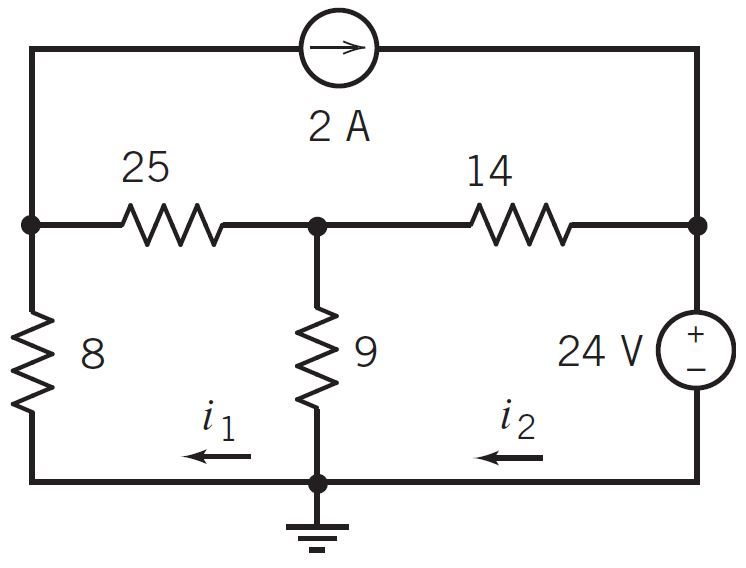
\includegraphics[width=.4\textwidth]{figuraP4_95.JPG}\\	
		\end{center}	
	%	\scalebox{0.8}{Answer: $i_{3}=\frac{13}{4}$ and $i_{2}=\frac{33}{4}$}
		\end{column}
	\end{columns}
\end{tabular}
\end{frame}

% ----------------- NOVA SECÇÂO -----------------------------
\section{Mesh Current Analysis with Dependent Sources (4.7)}
% ----------------- NOVO SLIDE --------------------------------
\begin{frame}[fragile]
	\frametitle{ Mesh Current Analysis with Dependent Sources}

\begin{tabular}{ll}
	\begin{columns}[c]	\column{1\textwidth}

		When a circuit contains a dependent source, the controlling current or voltage of that dependent source must be expressed as a function of the mesh currents.
	\end{columns} \\
	\begin{columns}

		\begin{column}{0.5\textwidth}  %%<--- here
.\\
.\\
		\textbf{EXAMPLE 4.7-1} - Consider the circuit. Find the value of the voltage measured by the voltmeter.
		\begin{center}
    			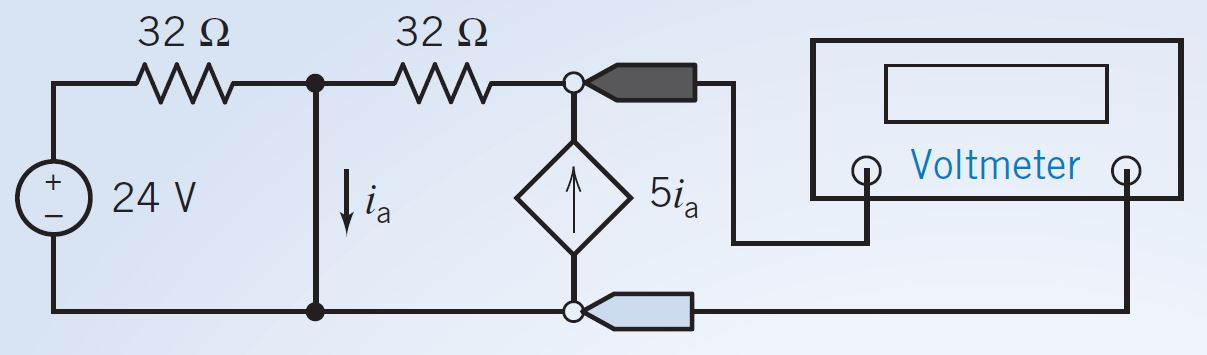
\includegraphics[width=1\textwidth]{figura4_71a.JPG}\\	
		\scalebox{0.8}{Answer: $v_{m}=30V$}

		\end{center}	
		\end{column}
		\begin{column}{0.7\textwidth}  %%<--- here
			\begin{equation}
			i_{a}=i_{1}-i_{2}
			\end{equation}
			\begin{equation}
			-i_{2}=5i_{a}=5(i_{1}-i_{2})
			\end{equation}
			\begin{equation}
			-24+32i_{1}=0
			\end{equation}
				\[ 
			\left[\begin{array}{rrr}
			5 & -4 \\		
			32 & 0  \end{array} \right]
			\left[\begin{array}{c}
			i_{1} \\		
			 i_{2}\end{array} \right]= 
			\left[\begin{array}{r}
			0 \\		
			24  \end{array} \right]
			\]	
		
		\end{column}
	\end{columns}\\
\end{tabular}


\end{frame}
% ----------------- NOVO SLIDE --------------------------------
\begin{frame}[fragile]

	\frametitle{Mesh Current Analysis with Current and Voltage Sources}
\begin{tabular}{ll}
	\begin{columns}
		\begin{column}{1\textwidth}  %%<--- here
		\textbf{PROBLEM 4.7-7} - The currents $i_{1}$, $i_{2}$, and $i_{3}$ are the mesh currents of the
circuit shown. Determine the values of $i_{1}$, $i_{2}$, and $i_{3}$.
		\begin{center}
    			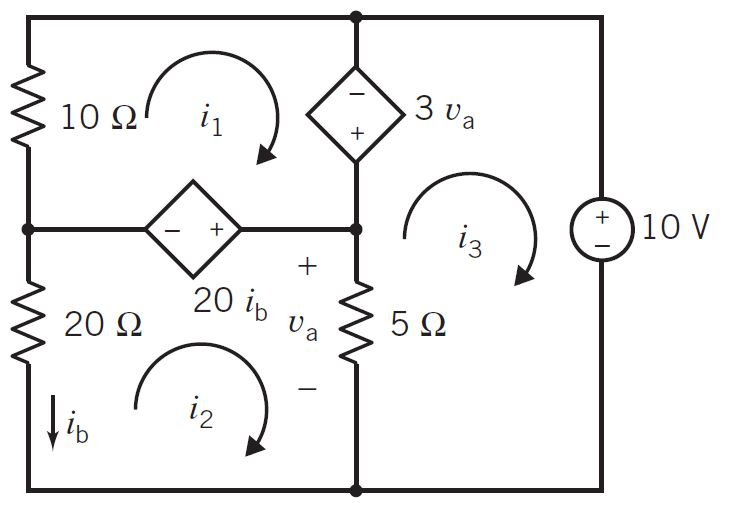
\includegraphics[width=.4\textwidth]{figuraP4_77.JPG}\\	
		\end{center}	
	%	\scalebox{0.8}{Answer: $i_{3}=\frac{13}{4}$ and $i_{2}=\frac{33}{4}$}
		\end{column}
	\end{columns}
\end{tabular}
\end{frame}

% ----------------- NOVA SECÇÂO -----------------------------
\section{The Node Voltage Method and Mesh Current Method Compared (4.8)}
% ----------------- NOVO SLIDE --------------------------------
\begin{frame}[fragile]
	\frametitle{ The Node Voltage Method and Mesh Current Method Compared}
	\begin{tabular}{cc}
			\begin{columns}
				\begin{column}{1\textwidth}  %%<--- here
					In some cases, one method is clearly preferred over another. For example:	\newline
		
					\begin{itemize}
						\item[$\clubsuit$] {When the circuit contains
only voltage sources, it is probably easier to use the mesh current method.}
						\item[$\clubsuit$] {When the circuit contains only
current sources, it will usually be easier to use the node voltage method.}						
					\end{itemize}
				.
				\end{column}
			\end{columns}
		
	\end{tabular}
\end{frame}
% ----------------- NOVO SLIDE --------------------------------
\begin{frame}[fragile]
	\frametitle{ The Node Voltage Method and Mesh Current Method Compared}
	\begin{tabular}{cc}
			\begin{columns}
				\begin{column}{1\textwidth}  %%<--- here
					If a circuit has both current sources and voltage sources, it can be analyzed by either method. One
approach is to compare the number of equations required for each method.	\newline
		
					\begin{itemize}
						\item[$\clubsuit$] {If the circuit has fewer nodes
than meshes, it may be wise to select the node voltage method.}
						\item[$\clubsuit$] {If the circuit has fewer meshes than
nodes, it may be easier to use the mesh current method.}						
					\end{itemize}
				.
				\end{column}
			\end{columns}
		
	\end{tabular}
\end{frame}
% ----------------- NOVO SLIDE --------------------------------
\begin{frame}[fragile]
	\frametitle{ The Node Voltage Method and Mesh Current Method Compared}
	\begin{tabular}{cc}
			\begin{columns}
				\begin{column}{1\textwidth}  %%<--- here
					Another point to consider when choosing between the two methods is what information is
required.	\newline
		
					\begin{itemize}
						\item[$\clubsuit$] {If you need to know several currents, it may be wise to proceed directly with mesh current analysis.}
						\item[$\clubsuit$] {If you need to know several voltages, it may be wise to proceed directly with node voltage  analysis.}						
					\end{itemize}
				.
				\end{column}


			\end{columns}\\
			\begin{columns}
			\begin{column}{1\textwidth} 
			It is often helpful to determine which method is more appropriate for the problem requirements
			and to consider both methods.
			\end{column}
			\end{columns}
	\end{tabular}
\end{frame}
% ----------------- NOVA SECÇÂO -----------------------------
\section{Circuit Analysis Using MATLAB (4.9)}
% ----------------- NOVO SLIDE --------------------------------
\begin{frame}[fragile]
	\frametitle{ Circuit Analysis Using MATLAB}




\begin{tabular}{ll}
	\begin{columns}[c]	\column{1\textwidth}
		In this section, we will use the MATLAB computer program to solve the equations.
	\end{columns} \\
	\begin{columns}
		\begin{column}{0.4\textwidth}  %%<--- here
		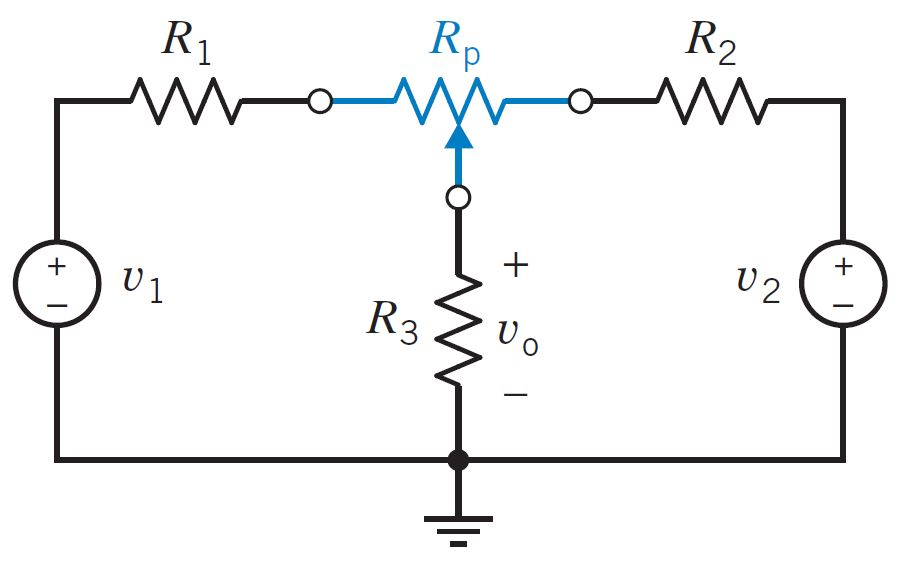
\includegraphics[width=1\textwidth]{figura4_91.JPG}\\	

		\scalebox{.6}{$\ R_{1} = 1000\Omega, \  R_{2} = 1000\Omega, \ R_{3}=5000\Omega, \ v_{1}=-v_{2}=15 V \ and \ R_{p}=20.000 \Omega$}
		\end{column}
		\begin{column}{0.6\textwidth}  %%<--- here
		{We have seen that circuits that contain resistors and independent or dependent sources can be analyzed
in the following way:}\\

					\begin{itemize}
						\item[$\clubsuit$] {Writing a set of node equations.}
						\item[$\clubsuit$]  {Solving those equations simultaneously.}
						
					\end{itemize}
		\end{column}
	\end{columns}
\end{tabular}






\end{frame}



\end{document} 